{\small
\section{Collections $\rightarrow$ Nur Referenzdatentypen ablegbar}{\label{Collections}}
    Beim Hinzufügen des Elements:\\
    Objekt selber \textbf{nicht} kopiert, nur eine Referenz wird abgelegt.

    \begin{tabular}{l l l}
        Grundlegende &$\cdot$ \textbf{List} & Folge von Elementen \\
        Collections: &$\cdot$ \textbf{Set}  & Menge von Elementen \\
                    &$\cdot$ \textbf{Map}  & Abbildung Schlüssel $\rightarrow$ Werte \\
    \end{tabular}

\subsection{Asymptotisches Laufzeitverhalten}
    \begin{tabularx}{\linewidth}{l l X} \hline
        \textbf{Laufzeit} & \textbf{Beschr.} & \textbf{Beispiele} \\ \hline
        O(1)        & Konstant      & Indexzugriff Array \\
        O(log(n))   & Logarithmisch & Binärsuche \\
        O(n)        & Linear        & Lineare Suche \\
        O(n*log(n)) & LogLinear     & Schnelle Sortierverfahren: QuickSort, MergeSort \\
        O(n$^2$)    & Quadr.        & Einfache Sortierverfahren: SelectionSort, InsertionSort \\
        O(n$^3$)    & Kubisch       & Matrizen-Multiplikation \\
    \end{tabularx}
    \vspace{-0.1cm}

    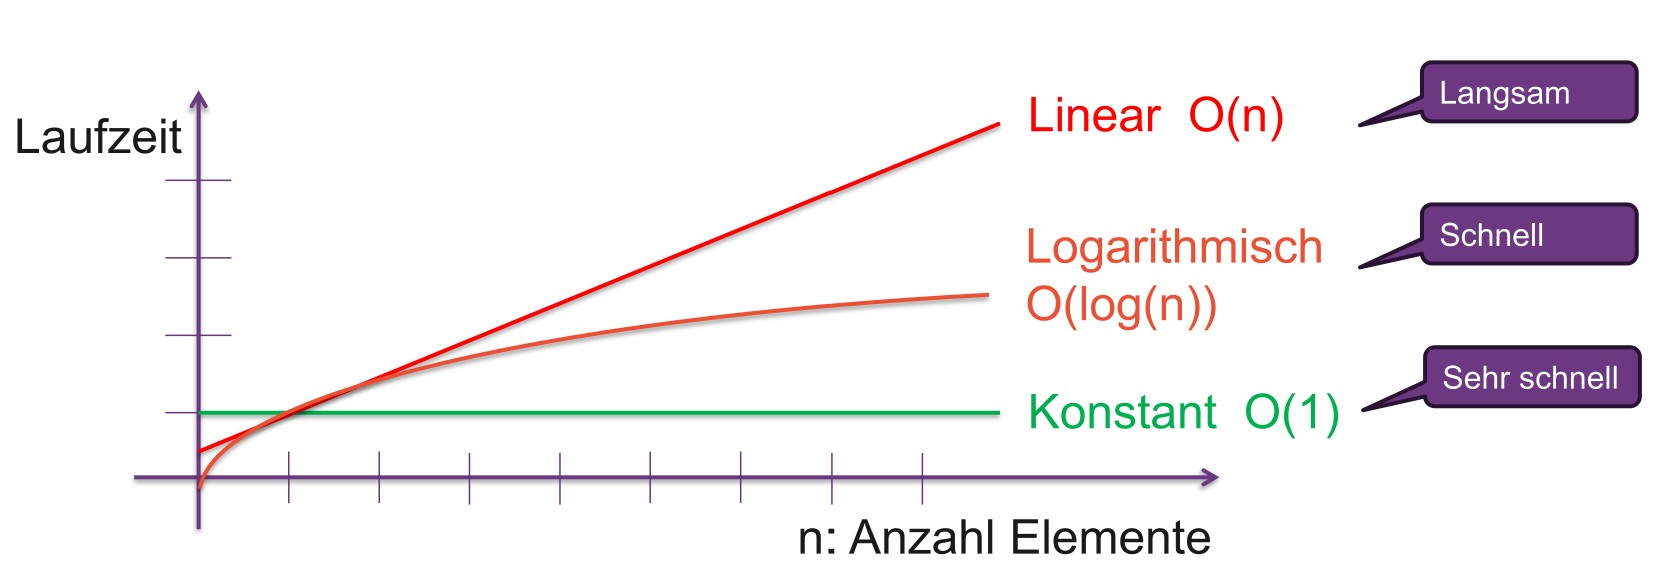
\includegraphics[width=\columnwidth]{pictures/laufzeit-collections.jpg}
    \vspace{-0.5cm}

\subsection{Wrapper-Objekt}
    Um primitive Datentypen in Collections verwenden zu können, müssen sie verpackt (\textit{Wrapping}) werden. Dies geschieht
    meist \textbf{implizit}, es muss nur beim Datentyp der Collection definiert werden.\\
    \vspace{-0.3cm}
    \begin{center}
        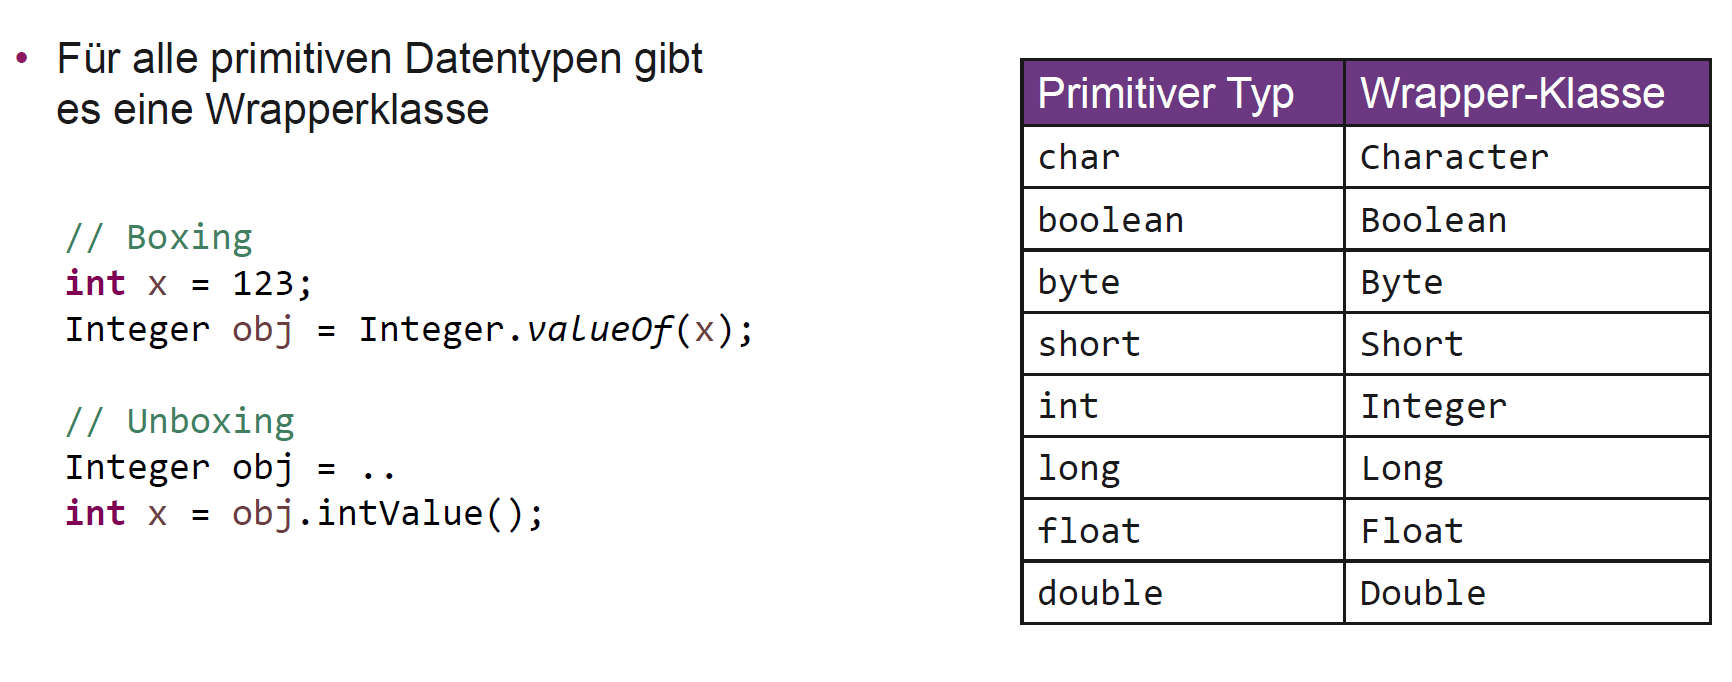
\includegraphics[width=0.85\columnwidth]{pictures/wrapper-klassen.png}
    \end{center}
    \vspace{-0.5cm}

\subsection{ArrayList}
    \begin{tabular}{l}
        $\bullet$ geordnete Folge von Elementen mit demselben Referenzdatentyp\\
        $\bullet$ Elemente können einfach hinzugefügt oder entfernt werden.\\
        $\bullet$ Duplikate oder \verb|null|-Einträge sind möglich\\
        $\bullet$ Zugriff auf Elemente erfolgt über Index (0 ... size()-1).\\
        $\bullet$ Die Liste verwendet intern ein Array zur Verwaltung der Elemente.\\
        $\bullet$ Zu Beginn enthält sie, sofern nicht anders definiert, 10 Elemente\\
        $\bullet$ Wird bei Erreichen der Kapazität mit Faktor 1.5 mulitpliziert.\\
    \end{tabular}

    \vspace{-0.1cm}
    \begin{center}
        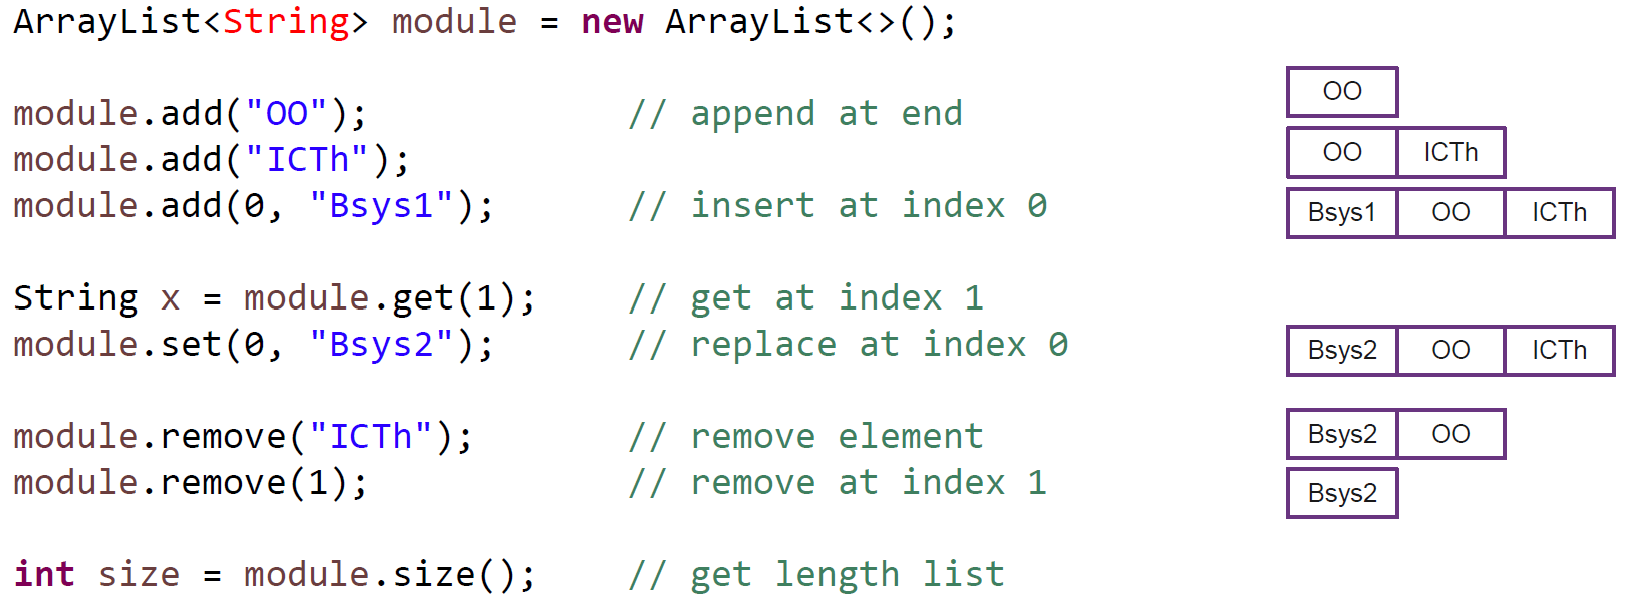
\includegraphics[width=0.78\columnwidth]{pictures/arrayList-bsp.png}
    \end{center}
    \vspace{-0.1cm}

    {\scriptsize 
        \begin{tabular}{l l}
            \rowcolor[RGB]{239,239,239} 
            \textbf{Type} & \textbf{Method / Description} $\rightarrow$ s./spec. = specified, elem = element\\ \hline
            void                       & \texttt{add(int index, E elem)} $\rightarrow$ Inserts s. elem at s. pos. in this list. \\ \hline
            boolean                    & \texttt{add(E e)} $\rightarrow$ Appends the spec. elem to the end of this list. \\ \hline
            boolean                    & \texttt{addAll(int index, Collection<? extends E> c)} $\rightarrow$ Inserts all elems\\
            & in spec. collection into this list, starting at spec. pos. \\ \hline
            boolean                    & \texttt{addAll(Collection<? extends E> c)} $\rightarrow$ Appends all elems in the\\
            & spec. collection to the end of this list, in the order\\
            & that they are returned by the spec. collection's Iterator. \\ \hline
            void                       & \texttt{clear()} $\rightarrow$ Removes all elems from this list. \\ \hline
            Object                     & \texttt{clone()} $\rightarrow$ Returns a shallow copy of this \texttt{ArrayList} instance. \\ \hline
            boolean                    & \texttt{contains(Object o)} $\rightarrow$ Returns \texttt{true} if list contains spec. elem \\ \hline
        \end{tabular}}
    \vspace{-0.1cm}

    \subsubsection{ArrayList: Kosten}
        {\small
        \begin{tabular}{l l l} \hline
            \textbf{Operation} & \textbf{Methode} & \textbf{Effizienz} \\ \hline
            Index-Zugriff & get(), set() & \color{green!80!black}Sehr schnell (direkter Zugriff) \\
            Hinzufügen    & add()        & \color{red}Langsam (umkopieren) \\
                        &              & \color{green!80!black}Sehr schnell (ohne umkop.) \\
            Entfernen     & remove(int)  & \color{red}Langsam (umkopieren) \\
            Finden        & contains()   & \color{red}Langsam (durchsuchen) \\
        \end{tabular}}
        \vspace{-0.1cm}

\subsection{LinkedList}
    Funktioniert ähnlich wie ArrayList. Die Implementierungerfolgt mit einer doppelt-verketteten (vor- und rückwärts) Liste.
    Es erfolgt kein Umkopieren beim Einfügen und Löschen von Elementen.
    \vspace{-0.1cm}

    \subsubsection{LinkedList: Kosten}
        {\small
        \begin{tabular}{l l l} \hline
            \textbf{Operation} & \textbf{Methode} & \textbf{Effizienz} \\ \hline
            Index-Zugriff & get(), set() & \color{red} Langsam (traversieren) \\
            Hinzufügen    & add()        & \color{green!80!black}Sehr schnell (Knoten einhängen)\\
            Entfernen     & remove(int)  & \color{red}Langsam in Mitte \\
                          &              & \color{green!80!black}Sehr schnell am Anfang und Ende \\
            Finden        & contains()   & \color{red}Langsam (traversieren) \\
        \end{tabular}}
        \vspace{-0.1cm}

\subsection{HashSet vs. TreeSet}
    \begin{tabular}{l}
        $\bullet$ Sets sind Container für Mengen\\
        $\bullet$ Duplikate \textbf{nicht} erlaubt\\
        $\bullet$ Gleichheit wird mit \verb|equals()| geprüft.\\
        $\bullet$ HashSets sind \textbf{unsortiert} und \textbf{oft sehr effizient}\\
        \verb|Set<String> firstSet = new HashSet<>();|\\
    \end{tabular}

    \begin{minipage}{0.5\columnwidth}
        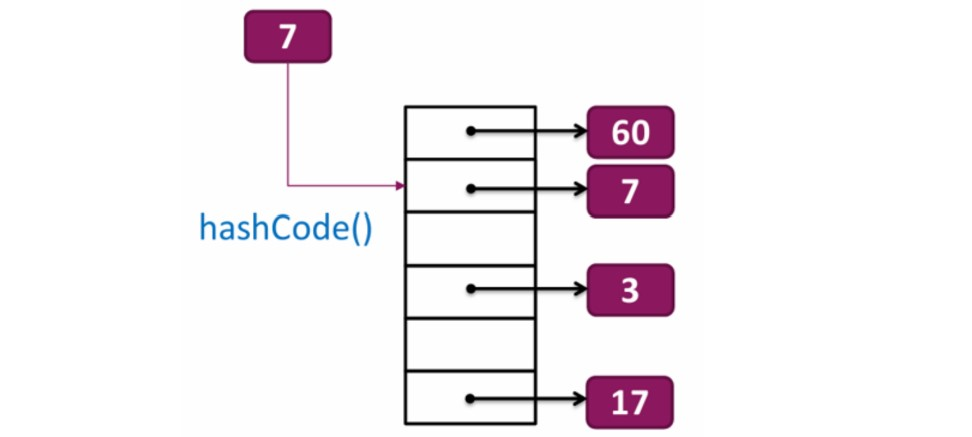
\includegraphics[width=0.9\linewidth]{pictures/hashset.jpg}
    \end{minipage}
    \hfill
    \begin{minipage}{0.45\columnwidth}
        Elemente liefern \verb|hashCode()| konsistent zu \verb|equals()|
    \end{minipage}

    TreeSets sind \textbf{sortiert} und \textbf{immer effizient}\\
    \verb|Set<String> firstSet = new TreeSet<>();|

    \begin{minipage}{0.5\columnwidth}
        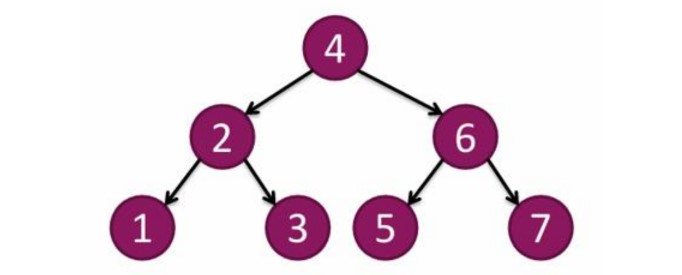
\includegraphics[width=0.9\linewidth-1cm]{pictures/treeset.jpg}
    \end{minipage}
    \hfill
    \begin{minipage}{0.45\columnwidth}
        Elemente impl. \verb|Comparable| und \verb|equals()|
    \end{minipage}
    \vspace{-0.1cm}

    \subsubsection{HashSet vs. TreeSet: Kosten}
        \begin{tabular}{l l l} \hline
            \textbf{Operation} & \textbf{TreeSet} & \textbf{HashSet }\\ \hline
            Finden      & \color{yellow!75!red} Schnell    & \color{green!80!black}Sehr schnell \\
            Einfügen    & \color{yellow!75!red} Schnell    & \color{green!80!black}Sehr schnell \\
            Löschen     & \color{yellow!75!red} Schnell    & \color{green!80!black}Sehr schnell (nur bei ``guter'' Impl.) \\
            Sortierung  & \color{green!80!black} Ja        & \color{red}Nein \\
        \end{tabular}
        \vspace{-0.1cm}

\subsection{HashMap vs. TreeMap}
    \begin{tabular}{l}
        $\bullet$ Maps sind für Mengen von Schlüssel-Wert-Paaren.\\
        $\bullet$ Jedem Schlüssel ist genau ein Wert zugeordnet.\\
        $\bullet$ \textbf{Keine} doppelten Schlüssel erlaubt. \\
    \end{tabular}

    \begin{center}
        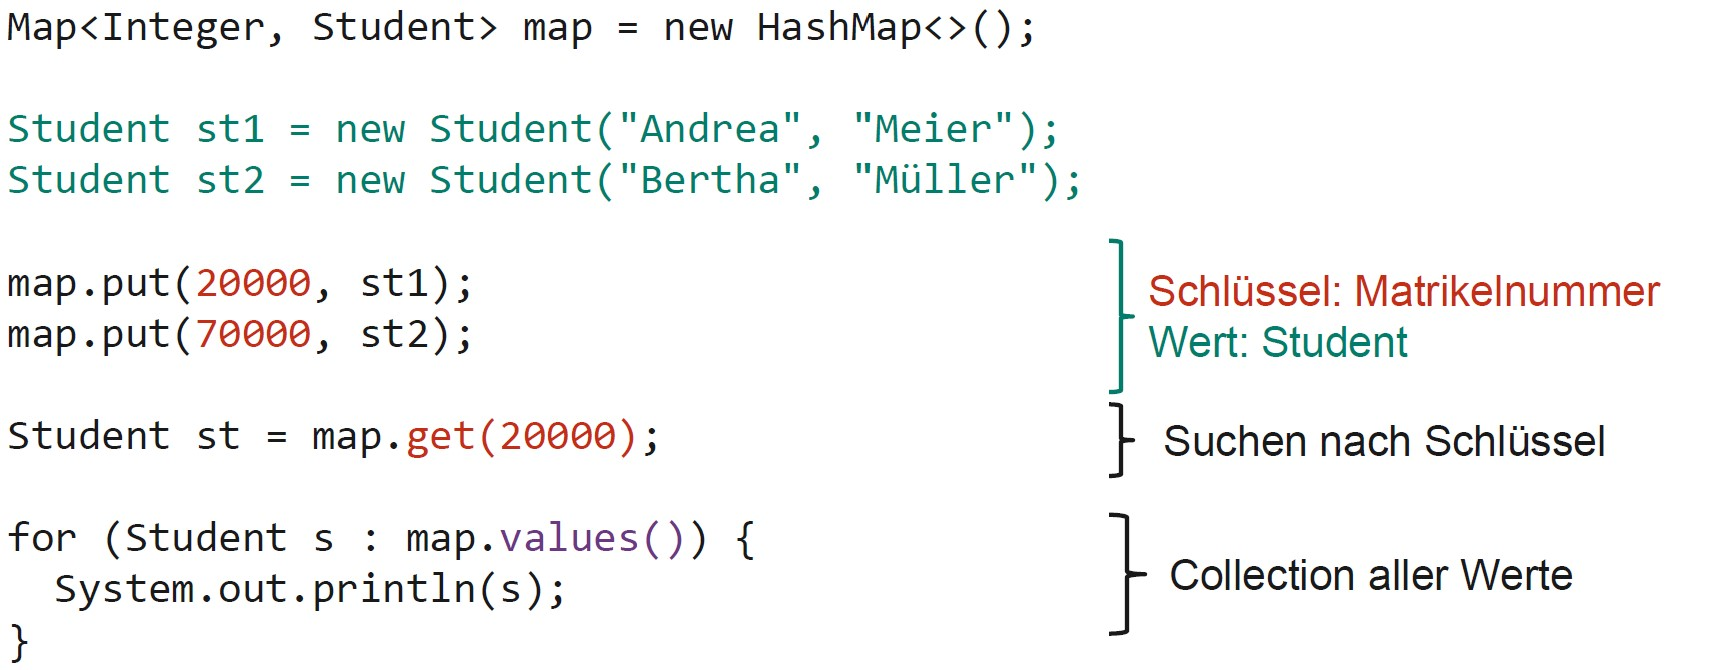
\includegraphics[width=0.85\linewidth]{pictures/map-beispiel.jpg}
    \end{center}

    \begin{tabular}{l}
        HashMaps sind \textbf{unsortiert} und \textbf{oft sehr effizient}\\
        \verb|Map<Integer, Student> masters = new HashMap<>();|\\
        \\   
        TreeMaps sind \textbf{nach Schlüssel sortiert} und \textbf{immer effizient}\\
        \verb|Map<Integer, Student> masters = new TreeMap<>();|\\
    \end{tabular}
    
    \columnbreak

    \subsubsection{HashMap vs. TreeMap: Kosten}
        \begin{tabular}{l l l} \hline
            \textbf{Operation} & \textbf{TreeMap} & \textbf{HashMap }\\ \hline
            Finden      & \color{yellow!75!red} Schnell             & \color{green!80!black}Sehr schnell \\
            Einfügen    & \color{yellow!75!red} Schnell             & \color{green!80!black}Sehr schnell \\
            Löschen     & \color{yellow!75!red} Schnell             & \color{green!80!black}Sehr schnell \\
                        &                                           & \color{green!80!black}(nur bei ``guter'' Impl.) \\
            Sortierung  & \color{green!80!black} Ja, nach Schlüssel & \color{red}Nein\\
        \end{tabular}
        \vspace{-0.1cm}

\subsection{equals(), Hashing}
    \begin{tabular}{ll}
        $\bullet$ & Operator \verb|==| liefert einen Referenzvergleich\\
        $\bullet$ & Methode \textbf{equals()} ist für den inhaltlichen Vergleich.\\
        $\bullet$ & Alle Klassen erben equals() von \textit{Object}.\\
                  & Die Default-Implementation liefert \verb|a == b| (Referenzvergleich).\\
        $\bullet$ & Bei einigen Klassen, z.B. \textit{String, Integer, ...} \\
                  & ist equals() bereits überschrieben.\\
        $\bullet$ & Eine Klasse \textbf{muss} equals() von \textit{Object} überschreiben:\\
    \end{tabular}

    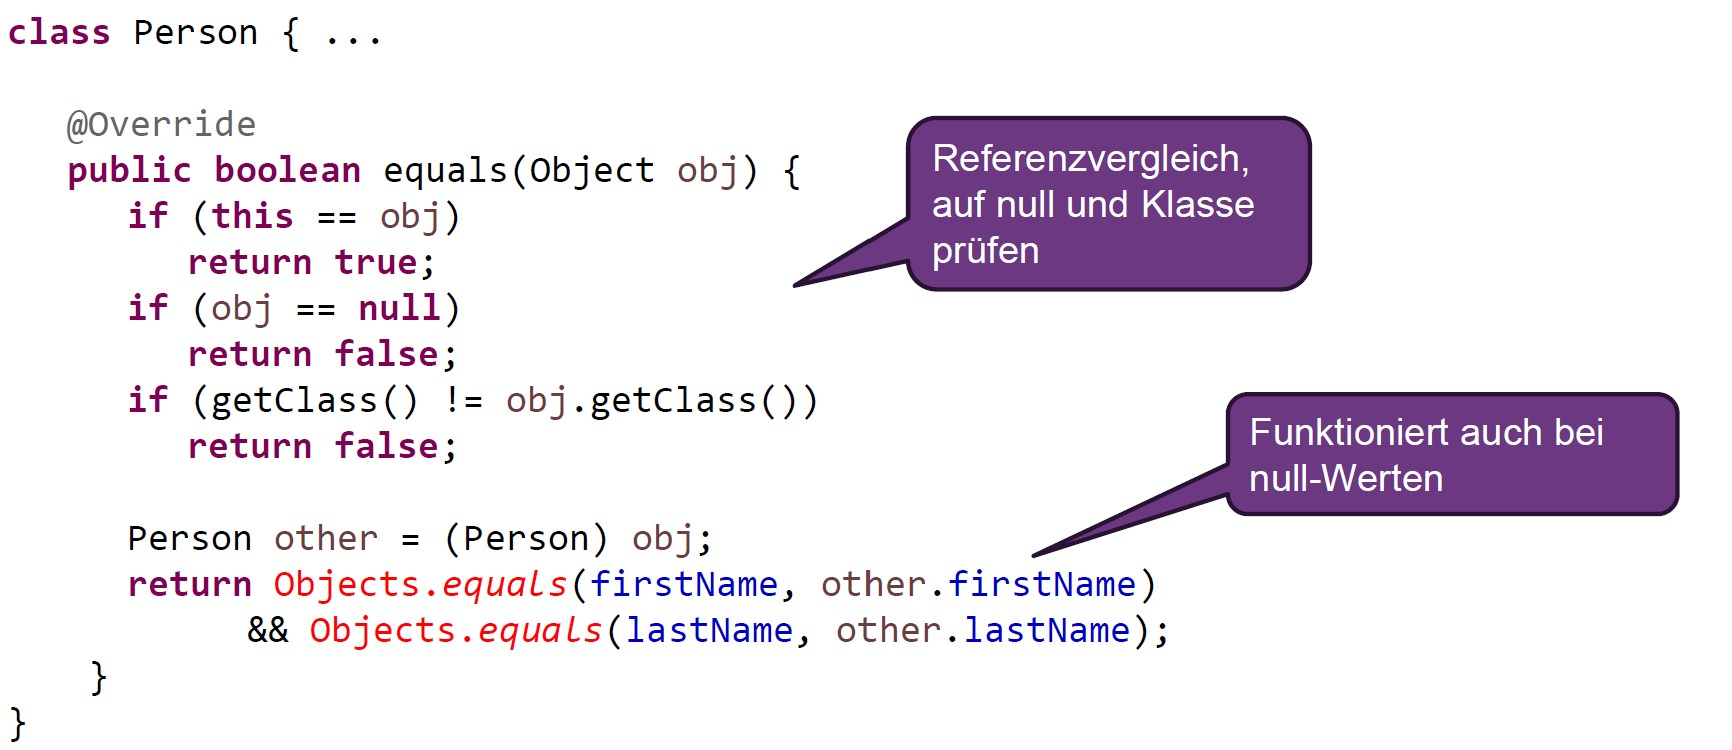
\includegraphics[width=\linewidth]{pictures/equals-impl.jpg}
    \vspace{-0.1cm}

    \subsubsection{Hashing: Konzept}
        \begin{tabular}{l}
            $\bullet$ Funktion \verb|hashCode()| bildet ein Objekt auf seinen Hash-Code ab,\\
            welcher den Ablegeort des Objekts definiert.\\
            $\bullet$ Gleiche Objekte können den gleichen Hashcode haben.\\
            \tikz[baseline=(text.base)]\node[fill=red, fill opacity=0.7, text opacity=1, rounded corners, inner sep=2pt, minimum height=5pt] (text) {\textit{Gleicher Hashcode muss aber nicht gleiches Objekt sein!}};\\    
        \end{tabular}
        \vspace{-0.1cm}

    \subsubsection{Hashfunktion $\rightarrow$ Für jedes equals() ein hashCode() schreiben}
        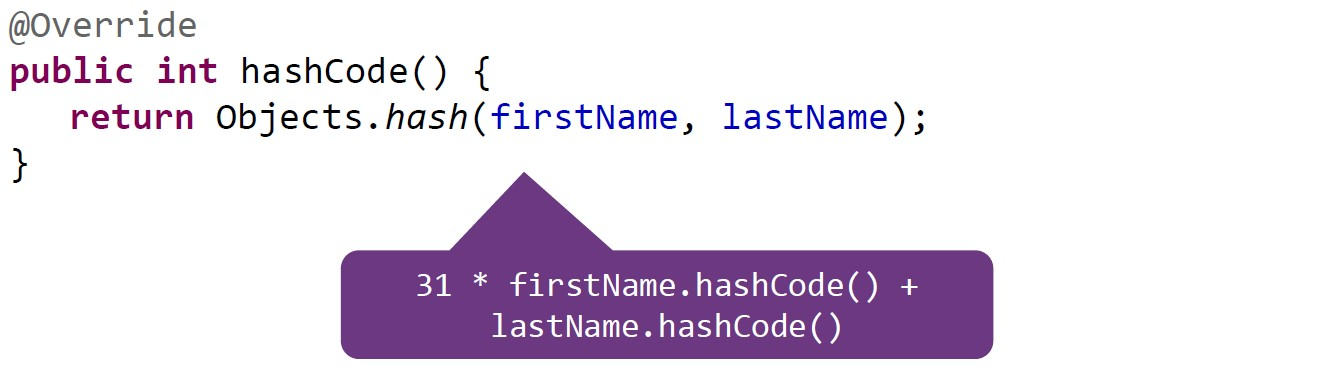
\includegraphics[width=0.9\linewidth]{pictures/hashcode.jpg}
        \vspace{-0.1cm}
}